\chapter{\label{chp:frameworkresults}Framework results}
The framework is tested using the reference design of a \gls{fir}-filter, described in \cref{subsec:refdesfir}. The source code of the filter, written in C, is listed in \cref{subsec:cfircode}. The implemented \gls{fir}-filter has a 32-bit input, 16 taps and 64-bit output. The filter-coefficients are for simplicity defined to be the integers 1-16. By running this design through the framework, multiple results will be generated. These results will be compared towards each other, but also towards the same \gls{fir}-filter implemented directly in Verilog. The source code of the Verilog implementation is listed in \cref{subsec:verilogfircode}. This testing will serve as a proof of concept, verifying the feasibility of the concept.

\section{\label{sec:firstrun}First test-run}
The first test-run was performed with 6 randomized constraints input to LegUp. Each of the constraints could take values 1 and 0, giving a total of $2^6=64$ combinations. The randomized constraints and the pattern of how the values are set is shown in \cref{tab:randomconstraint}.

\begin{table}
\tiny
    \begin{center}
    \begin{tabular}{l|cccccc}
     & & & \textbf{MB} & \textbf{ENABLE} & \textbf{DUAL} & \\
          &
          \textbf{SDC NO} & 
          \textbf{PIPELINE} & 
          \textbf{MINIMIZE} & 
          \textbf{PATTERN} & 
          \textbf{PORT} &
          \textbf{CASE} \\
        \textbf{Constraint}
           & \textbf{CHAINING}
           & \textbf{ALL}
           & \textbf{HW}
           & \textbf{SHARING}
           & \textbf{BINDING}
           & \textbf{FSM}
    \\ \midrule
    & 0 & 0 & 0 & 0 & 0 & 0 \\
    & 0 & 0 & 0 & 0 & 0 & 1 \\
    & 0 & 0 & 0 & 0 & 1 & 0 \\
    & 0 & 0 & 0 & 0 & 1 & 1 \\
    \textbf{Value} & \vdots & \vdots & \vdots & \vdots & \vdots & \vdots \\
    & &  &  &  &  &  \\
    & 1 & 1 & 1 & 1 & 1 & 0 \\
    & 1 & 1 & 1 & 1 & 1 & 1
    \\ \bottomrule
    \end{tabular}
    \caption{\label{tab:randomconstraint}Constraints and values for first run}
    \end{center}
\end{table}

This framework-run only include \gls{hls}, simulation, and synthesis, as the layout and power analysis tools have not yet been incorporated into the framework flow. Synthesis is run using a 32 MHz clock and a 180 nm cell library. A simple testbench generated by LegUp, with testcases similar to the ones listed in \cref{lst:tbcases}, were used for this run. 

The presented results are gathered from the synthesis reports. The generated Verilog-code for many of the constraint files synthesize into the exact same area and estimated power consumption. This indicates that some of the combinations are redundant. The results are shown in \cref{tab:hlsrun1dataresults}. As there are only 8 different results, only $log_2(8) = 3$ constraint parameters affect the design, the other will be don't-care constraints. By converting the design number to binary, a pattern can be seen. \Cref{tab:dectobinconstraints} shows the binary conversion of the design numbers at the second row of \cref{tab:hlsrun1dataresults}. Here it can be seen that the parameters \textit{PIPELINE\_ALL}, \textit{ENABLE\_PATTERN\_SHARING} and \textit{DUAL\_PORT\_BINDING} are don't care for this design, since these parameters are not constant.

The area results are given in cell units, dynamic and total power are given in milliWatts (mW), and leakage power is given in nanoWatts (nW).


\begin{table}[hbtp]
    \centering
    \begin{tabular}{ccccc}
    & & \multicolumn{3}{c}{\textbf{Power}} \\
    \cline{3-5}
    \textbf{Design \#} & \textbf{Area} & \textbf{Dynamic} & \textbf{Leakage} & \textbf{Total} \\
    \toprule
    Verilog & 175517.771501 & 2.9522 & 13.2559 & 2.9522 \\
    9,11,13,15,25,27,29,31 & 542636.067533 & 1.1933 & 445.5482 & 1.1937 \\
    8,10,12,14,24,26,28,30 & 543715.713936 & 1.1909 & 442.7919 & 1.1913 \\
    41,43,45,47,57,59,61,63 & 570759.857112 & 1.3097 & 474.8710 & 1.3102 \\
    1,3,5,7,17,19,21,23 & 571069.521032 & 1.2792 & 467.3262 & 1.2797 \\
    0,2,4,6,16,18,20,22 & 574368.902419 & 1.2745 & 467.3031 & 1.2750 \\
    40,42,44,46,56,58,60,62 & 574468.505099 & 1.3100 & 475.3570 & 1.3105 \\
    33,35,37,39,49,51,53,55 & 598731.305489 & 1.3951 & 498.4164 & 1.3956 \\
    32,34,36,38,48,50,52,54 & 599552.442242 & 1.3949 & 500.0916 & 1.3954 \\
    \bottomrule
    \end{tabular}
    \caption{Results from 1. framework-run}
    \label{tab:hlsrun1dataresults}
\end{table}

\begin{table}[hbtp]
    \centering
    \begin{tabular}{cccc}
    \textbf{Decimal} & \textbf{Binary}\\
    \toprule
    9 & 001001 \\
    11 & 001011 \\
    13 & 001101 \\
    15 & 001111 \\
    25 & 011001 \\
    27 & 011011 \\
    29 & 011101 \\
    31 & 011111 \\
    \bottomrule
    \end{tabular}
    \caption{Decimal to binary conversion of design numbers}
    \label{tab:dectobinconstraints}
\end{table}

\begin{figure}[hbpt]
\centering
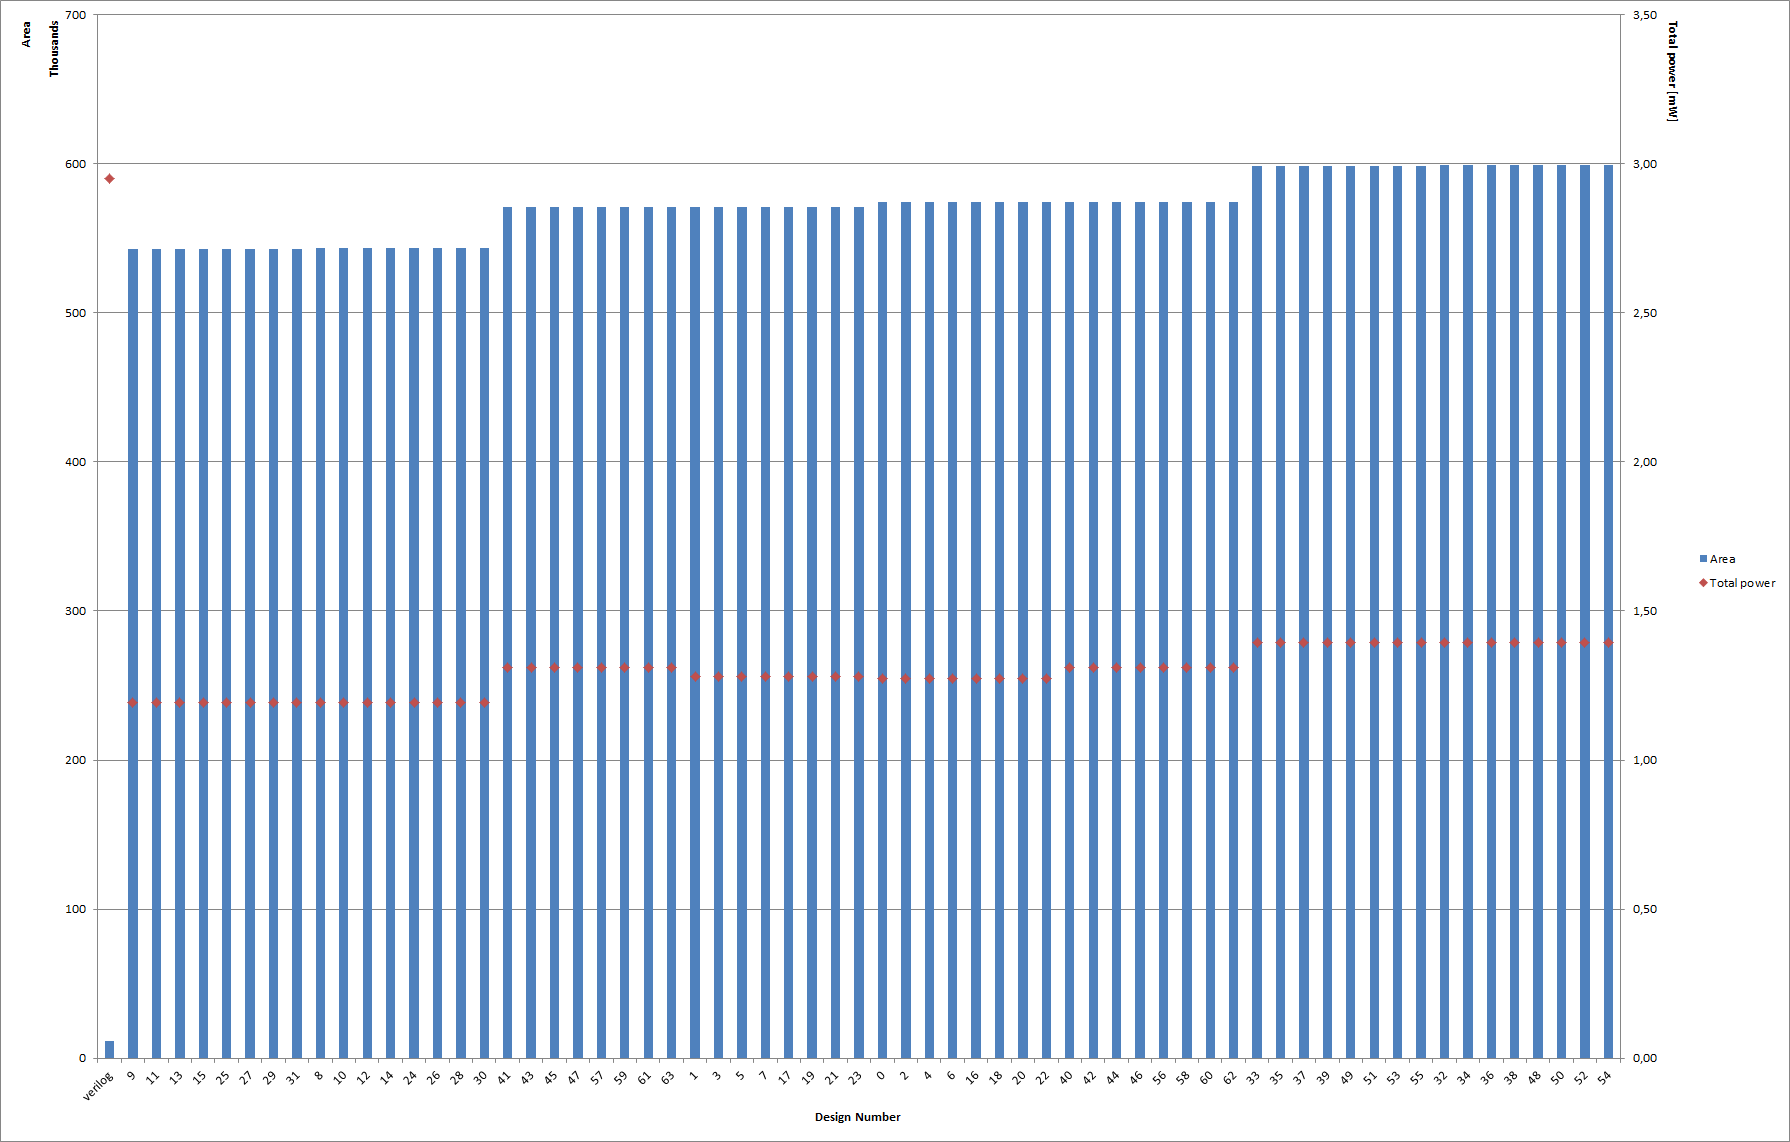
\includegraphics[width=\textwidth]{../figs/resultGraph.png}
\caption{\label{fig:resultgraphhlsrun1}Results from 1. framework-run}
\end{figure}
The best result with regards to area is the ones with the parameters \textit{SDC\_NO\_ CHAINING} set to 0, \textit{MB\_MINIMIZE\_HW} set to 1 and \textit{CASE\_FSM} set to 1. The best result with regards to total power consumption is the same as for area, but with \textit{CASE\_FSM} set to 0.

The results are visualized in \cref{fig:resultgraphhlsrun1}. It is clear from the graph that varying results are achieved from the different constraints. In \cref{fig:resultcomparisonhlsrun1}, the best area-result from the framework is compared towards the results from the same design written in Verilog directly. The design written directly in Verilog is better in terms of area, but it does not make sense that the estimated power consumption of the design written in Verilog is much higher than the \gls{hls}-generated design.

\begin{figure}[hbpt]
\centering
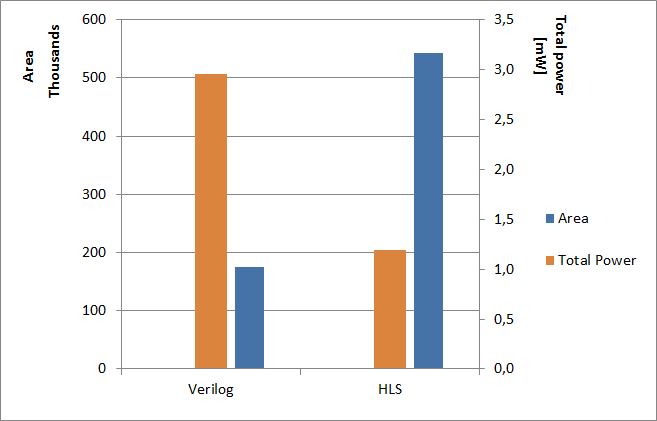
\includegraphics[width=0.75\textwidth]{../figs/resultComparison1.png}
\caption{\label{fig:resultcomparisonhlsrun1}Comparison of Verilog-design towards best HLS-design from 1. framework-run}
\end{figure}

\subsection{Handling unexpected results}
It seems strange that the area consumption of the design written in Verilog is just 32.3\% of the best result from LegUp, while the power consumption of the design written in Verilog is 247.4\% of the best result from LegUp. Typically a larger design will consume more power, as each of the components has leakage and static operation consumption. Notice that these results were obtained using a static power analysis tool. The amount of switching in gates and registers have not been taken into account. However, this unexpected result needed to be investigated further. The following steps were taken to ensure the quality of the results to be acceptable:

\begin{itemize}
    \item Check generated reports for misinterpreted data
    \item Look at schematic view of synthesized design to find errors
    \item Run \gls{hls} and synthesis once more to see if results deviates
\end{itemize}

None of the two first steps showed any errors. The designs are however too large to make any sense of the schematics, and due to to the limitation in setting signal sizes in the C-code, the \gls{hls}-generated designs scale down very poorly. The third step was performed on the same design, but with the clock relaxed from 32 MHz to 16 MHz. Changing the clock should not affect the design that much, but the synthesis will try to optimize the circuit to use the least amount of area, but still meet timing requirements. This time, only the constraints that had an impact on the design were included, generating 8 different designs. The result of the second run is shown in \cref{tab:resultgraphframeworkrun2} and in \cref{fig:resultgraphframeworkrun2}.
\begin{table}[hbtp]
    \centering
    \begin{tabular}{ccccc}
    & & \multicolumn{3}{c}{\textbf{Power}} \\
    \cline{3-5}
    \textbf{Design \#} & \textbf{Area} & \textbf{Dynamic} & \textbf{Leakage} & \textbf{Total} \\
    \toprule
    Verilog & 175531.077145 & 1.0961 & 291.4545 & 1.0964 \\
    3 & 736221.630958 & 3.0417 & 600.7903 & 3.0423 \\
    2 & 738362.360388 & 3.0424 & 603.0359 & 3.0430 \\
    0 & 766630.553023 & 3.1736 & 627.3008 & 3.1742 \\
    1 & 783120.518084 & 3.2230 & 641.3857 & 3.2236 \\
    7 & 796905.744222 & 3.0702 & 634.3779 & 3.0708 \\
    6 & 798087.595262 & 3.0693 & 635.5286 & 3.0699 \\
    4 & 830305.921961 & 3.2036 & 660.1381 & 3.2043 \\
    5 & 853504.409992 & 3.2898 & 681.0897 & 3.2905 \\

    \bottomrule
    \end{tabular}
    \caption{Results from 2. framework-run}
    \label{tab:resultgraphframeworkrun2}
\end{table}

\begin{figure}[hbpt]
\centering
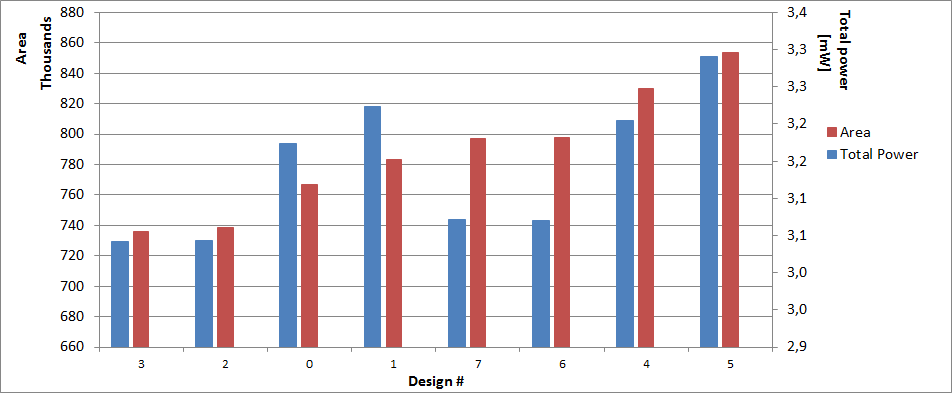
\includegraphics[width=\textwidth]{../figs/resultGraph2.png}
\caption{\label{fig:resultgraphframeworkrun2}Results from 2. framework-run}
\end{figure}

These results are a better match with our expectations. Both area and power has increased a bit for all \gls{hls}-generated designs. The reason for this is not known for sure, but it is possible that synthesis use larger library-cells to meet timing requirements. All timing requirements were not met in the first run, as described in \cref{sec:pathholdviolations}, which could lead to synthesis giving up and reporting a smaller area. It could also have been a bug in the design or a wrong setting in the first run that generated odd results. When comparing the best \gls{hls}-result towards the design written in Verilog, as shown in \cref{fig:resultcomparisonhlsrun2}, we see that the Verilog design has both lower area and power consumption, which is what would be expected.

\begin{figure}[hbpt]
\centering
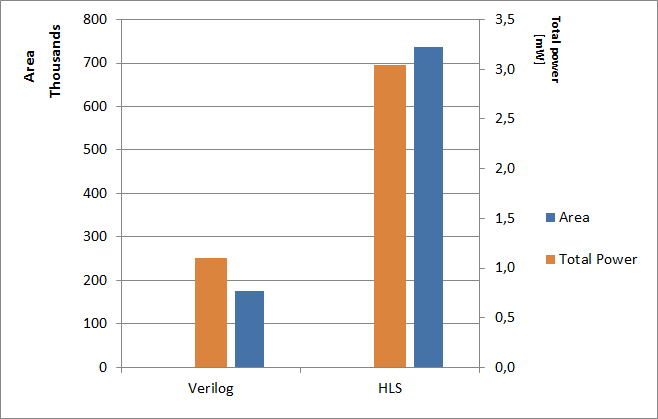
\includegraphics[width=0.75\textwidth]{../figs/resultComparison2.png}
\caption{\label{fig:resultcomparisonhlsrun2}Comparison of Verilog-design towards best HLS-design from 2. framework-run}
\end{figure}

\section{\label{sec:fullflowresults}Full tool-flow framework run}
The full tool-flow was incorporated into the framework, to see if the more accurate power analysis tool shows a different result. With the full tool-flow, the area reports are gathered from layout instead of synthesis and the power estimates are gathered from the power analysis. The full tool-flow is run using the same design as in \cref{sec:firstrun}, with only the three constraints that affected the output, again a total of 8 designs. Since the full tool-flow use switching data from simulation to perform power analysis, the testbench used for simulation had to be changed to get more switching values. The new testbench applies 1000 random inputs to the input \textit{inData}. It waits for the flag \textit{iterationFinished} to be set before applying a new input. The full source code of this testbench is listed in \cref{subsec:firfiltertb}. The testbench for the design written in Verilog is almost exacly the same, just adapted to the correct signal names and instead of waiting for a flag, \textit{inData} is assigned a new value after 17 clock-cycles. The area results are shown in \cref{tab:resultgraphareaframeworkrun2} and the power estimates are shown in \cref{tab:resultgraphpowerframeworkrun2}.

\begin{table}[hbtp]
    \centering
    \begin{tabular}{cccc}
    & \multicolumn{3}{c}{\textbf{Area}} \\
    \cline{2-4}
    \textbf{Design \#} & \textbf{Combinational} & \textbf{Non-combinational} & \textbf{Total} \\
    \toprule
    Verilog & 72818.22296 & 44647.6792 & 117465.9022 \\
    3 & 130953.7155 & 201114.5108 & 332068.2263 \\
    2 & 131389.4738 & 201114.5108 & 332503.9847 \\
    0 & 136182.8164 & 210973.9603 & 347156.7766 \\
    1 & 139276.3681 & 213895.2786 & 353171.6467 \\
    7 & 136262.6501 & 220468.2449 & 356730.8950 \\
    6 & 137237.2853 & 220468.2449 & 357705.5302 \\
    4 & 141315.4518 & 230327.6944 & 371643.1462 \\
    5 & 146770.7475 & 236170.3311 & 382941.0786 \\
    \bottomrule
    \end{tabular}
    \caption{Area results from full tool-flow framework-run}
    \label{tab:resultgraphareaframeworkrun2}
\end{table}

\begin{table}[hbtp]
    \centering
    \begin{tabular}{ccccc}
    & \multicolumn{4}{c}{\textbf{Power}} \\
    \cline{2-5}
    \textbf{Design \#} & \textbf{Net switching} & \textbf{Internal} & \textbf{Leakage} & \textbf{Total} \\
    \toprule
    Verilog & 0.365 & 1.760 & 100.340 & 2.125 \\
    2 & 1.214 & 5.157 & 281.820 & 6.371 \\
    3 & 1.236 & 5.270 & 273.940 & 6.507 \\
    6 & 1.184 & 5.484 & 293.960 & 6.669 \\
    0 & 1.273 & 5.518 & 292.400 & 6.792 \\
    1 & 1.279 & 5.517 & 307.760 & 6.797 \\
    7 & 1.255 & 5.567 & 267.960 & 6.822 \\
    4 & 1.238 & 5.696 & 308.180 & 6.934 \\
    5 & 1.269 & 5.771 & 327.280 & 7.041 \\
    \bottomrule
    \end{tabular}
    \caption{Power estimation results from full tool-flow framework-run}
    \label{tab:resultgraphpowerframeworkrun2}
\end{table}

In \cref{fig:resultgraphframeworkrun3} the final area and power estimation results are visualized together. It is clear from the graphs that the concept works, as we get different results from the designs. These results are considered more accurate, as they use the reports from the chip layout for area, and power estimation using switching activity from simulation. Notice that compared to the results from synthesis, the area is actually cut by half, but the estimated power consumption has nearly doubled. This is because the layout tool can run optimizations on the design, decreasing the area, while the power estimates takes the dynamic switching activity into account, increasing the total power consumption. In \cref{fig:resultcomparisonhlsrun3}, the area and power estimates from the full tool-flow framework-run is compared against the same design written directly in Verilog. Here we see the same trend as shown in the synthesis results above, but the relationship between area and power consumption shows more resemblance.

\begin{figure}[hbpt]
\centering
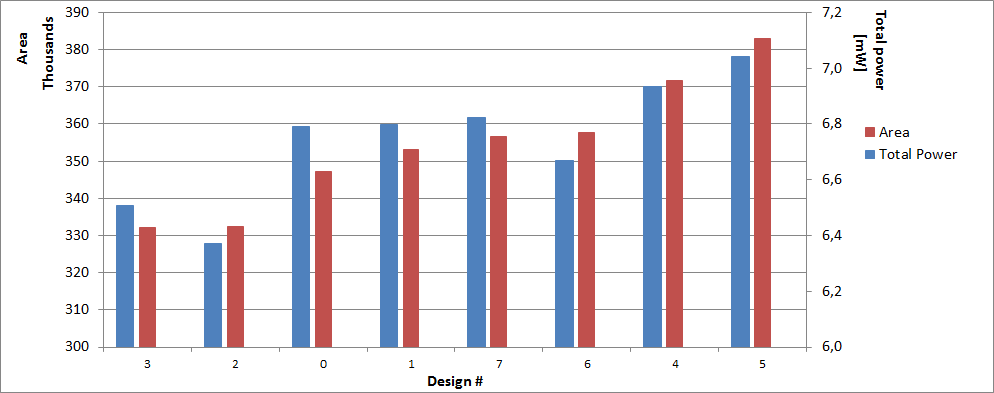
\includegraphics[width=\textwidth]{../figs/resultGraph3.png}
\caption{\label{fig:resultgraphframeworkrun3}Results from framework with full tool-flow}
\end{figure}

\begin{figure}[hbpt]
\centering
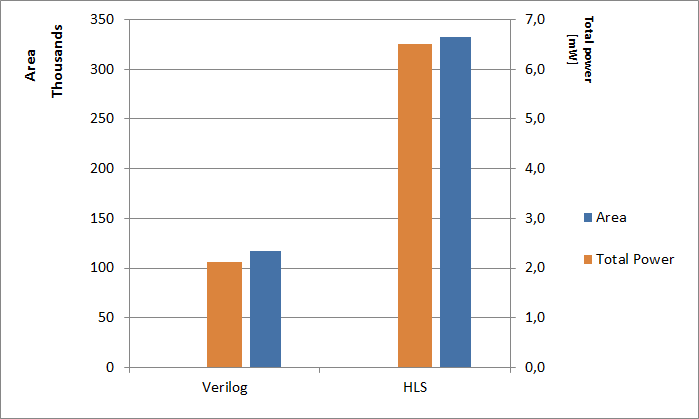
\includegraphics[width=0.75\textwidth]{../figs/resultComparison3.png}
\caption{\label{fig:resultcomparisonhlsrun3}Comparison of Verilog-design towards best HLS-design from full tool-flow framework-run}
\end{figure}

Figure \ref{fig:resultgraphareaframeworkrun2} and \ref{fig:resultgraphpowerframeworkrun2} shows the distribution of area and power consumption within the designs. In the power graphs, leakage power is not shown as this is negligible compared to the other factors. The trend is the same in all the \gls{hls} generated designs, the larger portion of the area is consumed by non-combinational area. In the Verilog designs, the area distribution is inverted. This difference is what is expected from a \gls{fsm} vs not-\gls{fsm} design. In the power distribution graph we see that most of the power is consumed internally in the cells both in \gls{hls} generated designs and the Verilog design.

\begin{figure}[hbpt]
\centering
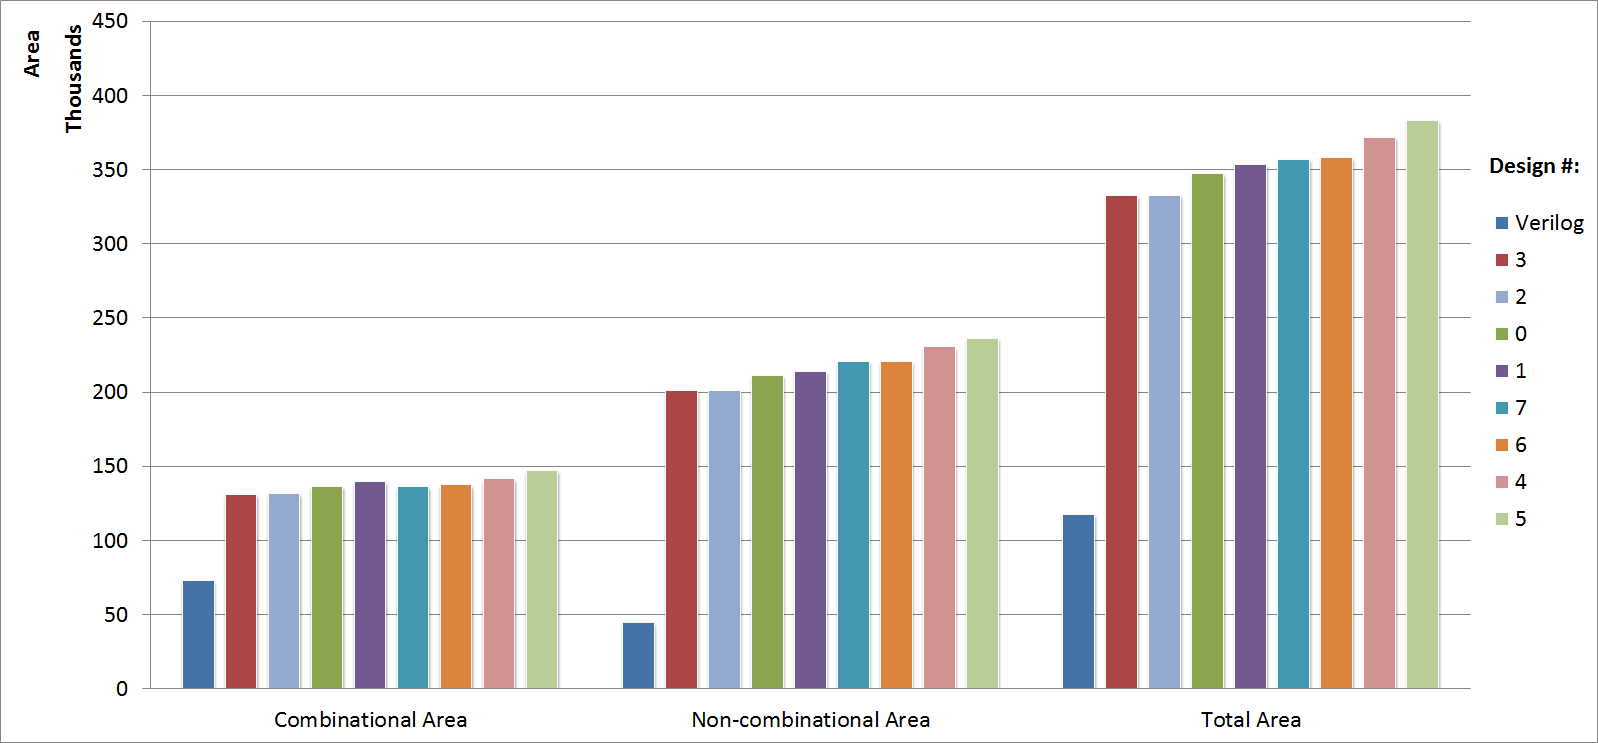
\includegraphics[width=\textwidth]{../figs/resultGraphAreaDistribution.png}
\caption{\label{fig:resultgraphareaframeworkrun2}Area distribution of results from framework with full tool-flow}
\end{figure}

\begin{figure}[hbpt]
\centering
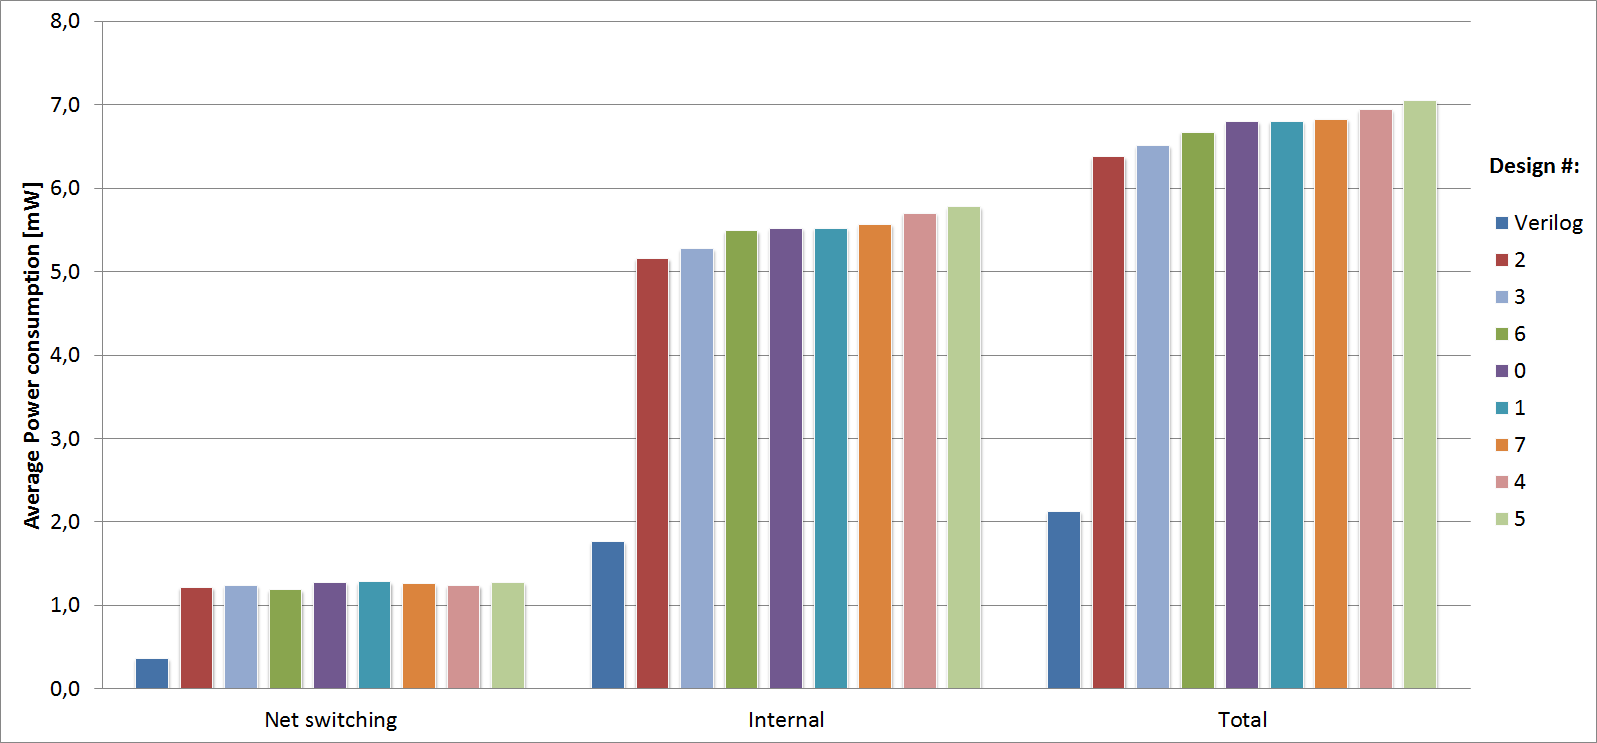
\includegraphics[width=\textwidth]{../figs/resultGraphPowerDistribution.png}
\caption{\label{fig:resultgraphpowerframeworkrun2}Power distribution of results from framework with full tool-flow}
\end{figure}

Two other interesting parameters to compare, is the number of generated registers, and the critical path and corresponding maximum frequency. For the implemented design, a minimum of 480 1-bit registers (\verb!INPUTSIZE*(TAPS-1)!) is needed for the shift register, the \textit{sr}-array. The number of registers, gathered from the synthesis reports, is shown in \cref{tab:resultregistercount}. 

\begin{table}[hbtp]
    \centering
    \begin{tabular}{cc}
    \textbf{Design \#} & \textbf{Registers} \\
    \toprule
    Verilog & 480 \\
    0 & 2311 \\
    1 & 2343 \\
    2 & 2203 \\
    3 & 2203 \\
    4 & 2523 \\
    5 & 2587 \\
    6 & 2415 \\
    7 & 2415 \\
    \bottomrule
    \end{tabular}
    \caption{Number of used registers from full framework run}
    \label{tab:resultregistercount}
\end{table}
The maximum speed of the designs can be calculated from the critical path length, reported in both synthesis and layout. The critical path is the longest path through the circuit, calculated as the summation of the delay of each logical cell. The maximum frequency of the design is given as:
\begin{equation}
   F_{MAX} = \frac{1}{t_{criticalPath}}
\end{equation}


The critical path results and corresponding F\textsubscript{MAX} is shown in \cref{tab:critpathfmax}. The results for the \gls{hls}-generated designs are quite similar, but notice the large gap down to the design written directly in Verilog. Here the overhead of the \gls{fsm} generated by LegUp is revealed. The synthesis and layout are setup to perform optimization of the area, while making sure the timing requirements of the target clock-period is met. This optimization goal can explain why the results are so similar for all designs. 
\begin{table}[hbtp]
    \centering
    \begin{tabular}{c|cc|cc}
     \multicolumn{1}{c}{} & \multicolumn{2}{c}{\textbf{Critical Path Length [nS]}} & \multicolumn{2}{c}{\textbf{F\textsubscript{MAX} [MHz]}}\\
     \cline{2-5}
     \textbf{Design \#} & \textbf{Synthesis} & \textbf{Layout} & \textbf{Synthesis} & \textbf{Layout} \\
    \toprule
    Verilog & 2.33 & 3.07 & 429.2 & 325.7 \\
    0 & 47.14 & 50.80 & 21.21 & 19.69\\
    1 & 47.28 & 52.33 & 21.15 & 19.11\\
    2 & 47.14 & 51.11 & 21.21 & 19.57\\
    3 & 47.22 & 51.77 & 21.18 & 19.32\\
    4 & 47.75 & 54.53 & 20.94 & 18.34\\
    5 & 49.23 & 54.66 & 20.31 & 18.30\\
    6 & 50.79 & 56.16 & 19.69 & 17.81\\
    7 & 50.11 & 53.70 & 19.96 & 18.62\\
    \bottomrule
    \end{tabular}
    \caption{Critical path length and maximum frequency results from full framework run}
    \label{tab:critpathfmax}
\end{table}
       
\section{\label{sec:designbugs}Bugs in the generated design}
To avoid the generation of a global memory controller, the flag \textit{NO\_INLINE} had to be set to 0 in the Makefile. This introduces two bugs in the generated Verilog; firstly, the signal generated from the parameter \textit{done} is not sampled after the first time, making the program run forever, secondly the statement \verb!products[0] = inData * 1! is only evaluated on the first iteration of the loop, meaning all outputs from the \gls{fir}-filter (except the first one) will have a deviation from the correct result, corresponding to \verb!correctResult - inData + firstInData!. From the generated LLVM \gls{ir}-code it looks like the first bug occurs because the comparison of the input \textit{done} being performed under another label than where it is used as exit-condition for the while-loop. Under the same label, \textit{inData} is sign-extended, as it is a 32-bit variable being assigned to a 64-bit variable. Both these results are stored to temporary registers for use later, as shown below. From the simulation, it can be seen that the states generated by these operations are not visited again when the loop has been entered. It looks to be the implemented method for supporting streaming inputs and outputs that is the source of these bugs. When calling a function in C, it is not expected that the input-parameters shall change during run-time. It is therefore reasonable that the compiler schedule these operations before entering the while-loop, to prevent doing the same work multiple times.
\lstset{language=llvm,style=LLVMstyle}
\begin{lstlisting}
%6 = icmp eq i32 %done, 0
%7 = sext i32 %inData to i64
\end{lstlisting}
These bugs are not critical to this proof of concept, as both bugs will be identical to every design. As these results are only supposed to show that the concept works, it is not critical that the generated results are accurate, as long as the fidelity of the results is high.
\section{\label{sec:pathholdviolations}Path and hold violations}
Some of the designs report violating path-length and hold-times in synthesis during 1. framework-run. For a real circuit this would be a problem. To get rid of these violations, the target clock speed during synthesis could be decreased to something below the maximum frequency of the design. However, the clock speed is most of the time the only thing you cannot change in your design, and the synthesis tool will try to create the circuit that meets timing. If timing is not met, the circuit description should be changed. This means that from our methodology, we will generate many circuits and only the ones that meet timing will be presented as an accepted solution. Ideally, the framework would implement a feedback loop, but for the sake of this proof of concept, a long list of solutions are produced and only the best ones are selected. No violations were reported during 2. or 3. framework-run.

\section{\label{sec:codeoptimization}LegUp specific code optimization}

When going trough the register-count from synthesis, it was noticed that the \gls{hls}-generated designs implemented both the array \textit{sr} and \textit{products} as \gls{ram} modules using registers. In the design written directly in Verilog, the \textit{sr}-array is the only consumer of registers. When looking at the following snippet from the \gls{fir}-filter source code, listed in \cref{subsec:cfircode}:
\lstset{language=C,style=CStyle}
\begin{lstlisting}
for (int k = 1; k < TAPS ; k++){
    products[k] = sr[k-1] * (k+1);
}
sum = sum + products[i];
\end{lstlisting}
it can easily be seen that this is functionally equivalent to:
\begin{lstlisting}
sum = sum + (sr[i-1] * (i+1));
\end{lstlisting}
It can be argued that the second listing is better C-code, but it would be natural to assume modern compilers could handle such optimizations automatically. This optimization should be done in the compiler or in LegUp, but it was not done either places.

If we also substitute the code:
\begin{lstlisting}
products[0] = inData * 1;
sum = products[0];
\end{lstlisting}
with:
\begin{lstlisting}
sum = inData * 1;
\end{lstlisting}
the whole \textit{products}-array can be removed. When running this optimized code through the framework, the result is much better than without these optimizations. Table \ref{tab:resultsframeworkrun3} shows the results from the framework run of design 2, the best design with regards to power consumption from the full tool-flow framework-run.

\begin{table}[hbtp]
    \centering
    \begin{tabular}{lr}
    \multicolumn{2}{c}{\textbf{Synthesis}} \\
    \toprule
    Total Area & 358587.628093 \\
    \hline
    Net Switching Power & 0.1340 mW \\
    Internal Power & 1.3203 mW \\
    Leakage Power & 283.1053 nW \\
    \hline
    Total Power & 1.4546 mW \\
    \hline
    Register count & 899 \\ 
    \bottomrule
    & \\
    \multicolumn{2}{c}{\textbf{Layout}} \\
    \toprule
    Combinational Area & 72482.256207 \\
    Non-combinational Area & 82070.787659 \\
    \hline
    Total Area & 154553.043866 \\
    \bottomrule
    & \\
    \multicolumn{2}{c}{\textbf{Power analysis}} \\
    \toprule
    Avg. Net Switching Power & 0.604 mW \\
    Avg. Internal Power & 2.413 mW \\
    Avg. Leakage Power & 105.500 nW \\
    \hline
    Avg. Total Power & 3.018 mW \\
    \bottomrule
    \end{tabular}
    \caption{Results of best design from framework run with optimized C-code.}
    \label{tab:resultsframeworkrun3}
\end{table}
The results from the optimized code gives the overhead shown in \cref{tab:overheadframeworkrun3}. These overhead percentages corresponds more with the typical overhead of 30-40\% in \gls{hls}-tools.
\begin{table}[hbtp]
    \centering
    \begin{tabular}{lr}
    \multicolumn{2}{c}{\textbf{Overhead}} \\
    \toprule
    %Synthesis area & 183056.550948 (104.29\%)
    %Synthesis power & 0.3582mW (32.67\%)
    %Register count & 419 1-bit registers (87.29\%)
    Layout area & 37087.141666 (31.57\%) \\
    Average power & 0.893mW (42.02\%) \\
    Register count & 419 (87.29\%) \\
    \bottomrule
    \end{tabular}
    \caption{Overhead from results of optimized C-code.}
    \label{tab:overheadframeworkrun3}
\end{table}

